\chapter{Sysmon Installation}

\section{Installation via \acrshort{gpo}}

Sysmon kann auf der \href{https://docs.microsoft.com/en-us/sysinternals/downloads/sysmon}{Webseite von Microsoft}\footnote{Link: https://docs.microsoft.com/en-us/sysinternals/downloads/sysmon} heruntergeladen werden.
Es gibt eine 32- und 64-Bit Version von Sysmon.

Zusätzlich braucht es noch eine Konfigurationsdatei welche definiert, was Sysmon in den Event Log schreibt.
Die Konfiugrationsdatei kann man im \href{https://github.com/KMU-Incident-Response/KMU-Basis-Logging}{KMU-Incident-Response Repository}\footnote{Link: https://github.com/KMU-Incident-Response/KMU-Basis-Logging} herunterladen.\\

Die .exe und .xml Dateien müssen in einem freigegebenen Netzlaufwerk abgespeichert werden, auf welches alle Windows Geräte Zugriff haben. Zum Beispiel auf dem Domain Controller unter:
\begin{lstlisting}
    C:\Windows\SYSVOL\sysvol\<Domain>
\end{lstlisting}

Nun muss eine neue Group Policy erstellt werden, mit welcher Sysmon auf den Windows Geräten installiert wird.
Dazu öffnet man das Group Policy Management auf dem Domain Controller und erstellt eine neue Group Policy, welche mit der \acrshort{ou} verknüpft ist, die alle Windows Geräte enthält.
\begin{figure}[H]
    \centering
    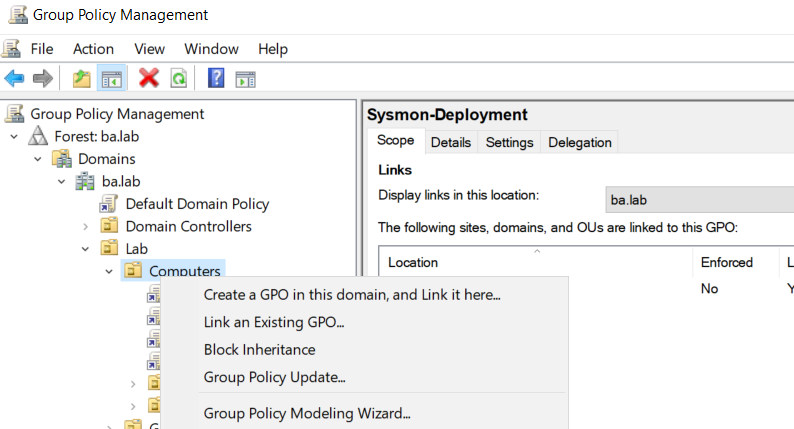
\includegraphics[width=0.7\linewidth]{../img/agent/create-new-group-policy.png}
    \caption{Neue Group Policy für Sysmon Deployment}
\end{figure}

Die Group Policy muss mit \textbf{Rechtsklick $\rightarrow$ Edit} bearbeitet werden.
Unter \textbf{Computer Configuration $\rightarrow$ Preferences $\rightarrow$ Windows Settings $\rightarrow$ Folder} kann mit \textbf{Rechtsklick $\rightarrow$ New $\rightarrow$ Folder} ein neuer Ordner auf den Windows Geräten angelegt werden.
Dieser wird benötigt, um die Dateien vom freigegebenen Netzlaufwerk in diesen Ordner zu kopieren.
Es müssen folgende Einstellungen vorgenommen werden:\\
\begin{minipage}{0.5\linewidth}
    \begin{figure}[H]
        \centering
        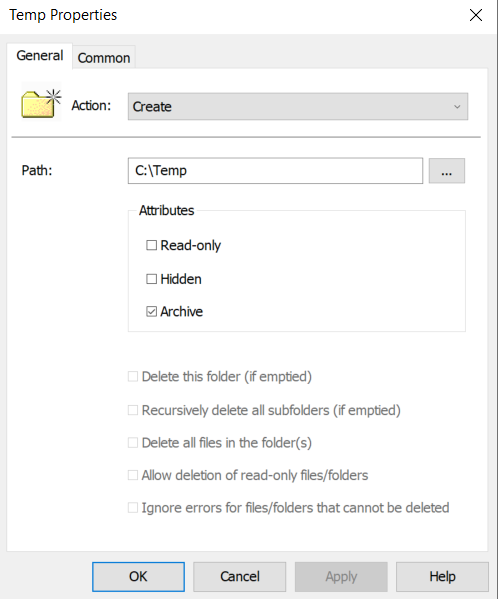
\includegraphics[width=0.7\linewidth]{../img/sysmon/new-folder-1.png}
        \caption{Neuer Ordner mit GP erstellen 1}
    \end{figure}
\end{minipage}
\begin{minipage}{0.5\linewidth}
    \begin{figure}[H]
        \centering
        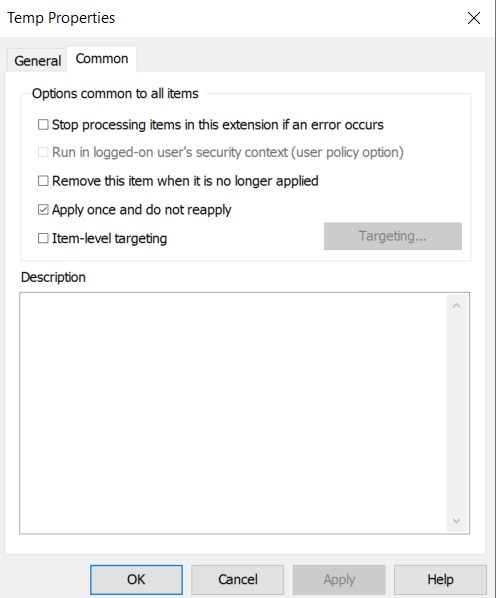
\includegraphics[width=0.7\linewidth]{../img/sysmon/new-folder-2.png}
        \caption{Neuer Ordner mit GP erstellen 2}
    \end{figure}
\end{minipage}\\

Danach kann man mit ``OK'' bestätigen.\\

Als nächstes wird das kopieren der Dateien eingerichtet.
Dazu macht man im Menu links auf Files \textbf{Rechtsklick $\rightarrow$ New $\rightarrow$ Files} und erstellt eine neue Policy.
Dies muss einmal für die .exe und zusätzlich für die .xml Datei gemacht werden.
Als \textbf{Action} wählt man ``Create''.
Als \textbf{Source File} wählt man die Dateien auf dem freigegebenen Netzlaufwerk.
Als \textbf{Destination File} wählt man den zuvor erstellten Ordner.
Unter dem Reiter \textbf{Common} muss wieder ein Hacken bei ``Apply once and do not reapply'' gesetzt werden:\\
\begin{minipage}{0.5\linewidth}
    \begin{figure}[H]
        \centering
        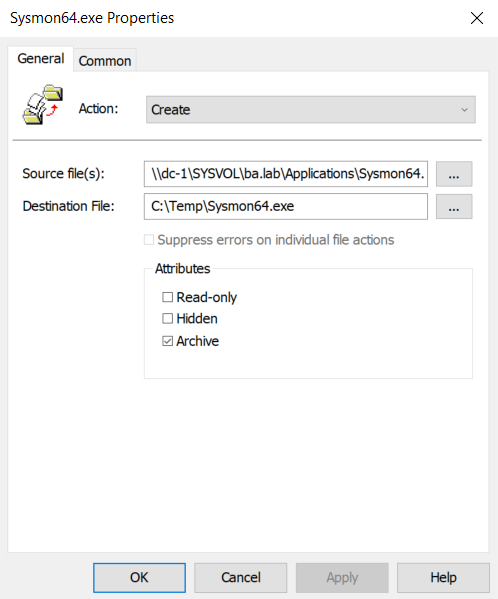
\includegraphics[width=0.7\linewidth]{../img/sysmon/sysmon-file.png}
        \caption{Sysmon.exe kopieren}
    \end{figure}

\end{minipage}
\begin{minipage}{0.5\linewidth}
    \begin{figure}[H]
        \centering
        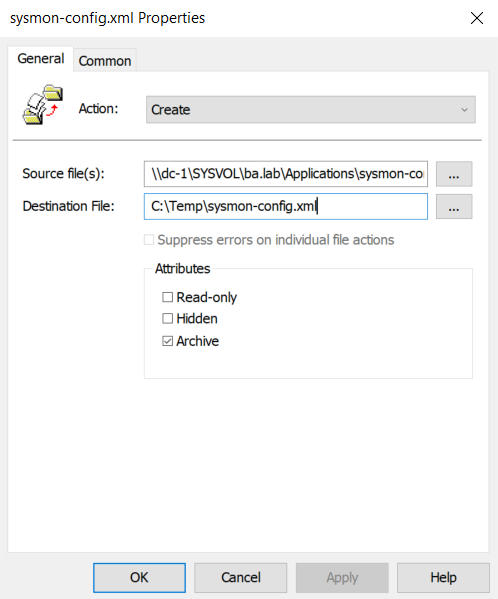
\includegraphics[width=0.7\linewidth]{../img/sysmon/config-file.png}
        \caption{sysmon-config.xml kopieren}
    \end{figure}
\end{minipage}

Zuletzt muss noch ein neuer Immediate Task unter \textbf{Computer Configuration $\rightarrow$ Preferences $\rightarrow$ Control Panel Settings $\rightarrow$ Scheduled Tasks} mit \textbf{Rechtsklick $\rightarrow$ New $\rightarrow$ Immediate Task (At least Windows 7)} erstellt werden.
\begin{figure}[H]
    \centering
    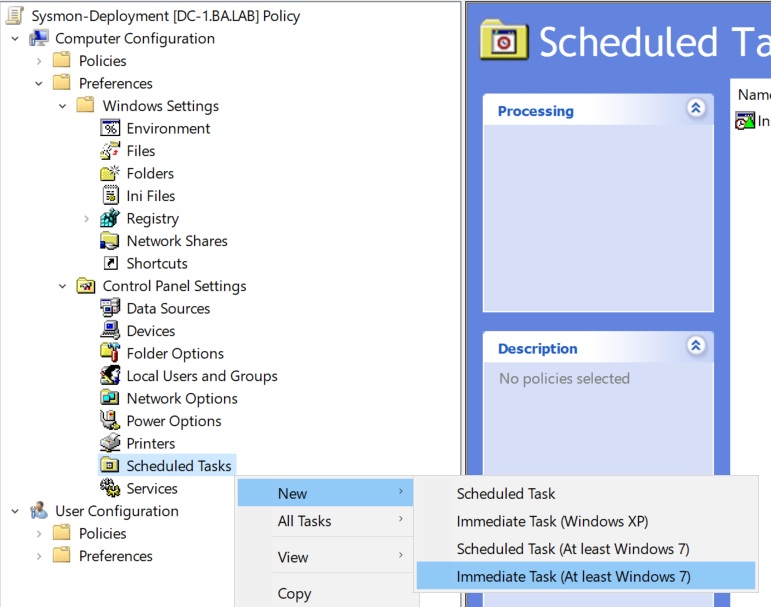
\includegraphics[width=0.7\linewidth]{../img/sysmon/new-scheduled-task.png}
    \caption{Neuen Immediate Task erstellen}
\end{figure}

Unter dem Reiter \textbf{Common} muss wieder ein Hacken bei ``Apply once and do not reapply'' gesetzt werden.
In den Reitern \textbf{General} und \textbf{Action} werden folgende Einstellungen getroffen:\\
\begin{minipage}{0.5\linewidth}
    \begin{figure}[H]
        \centering
        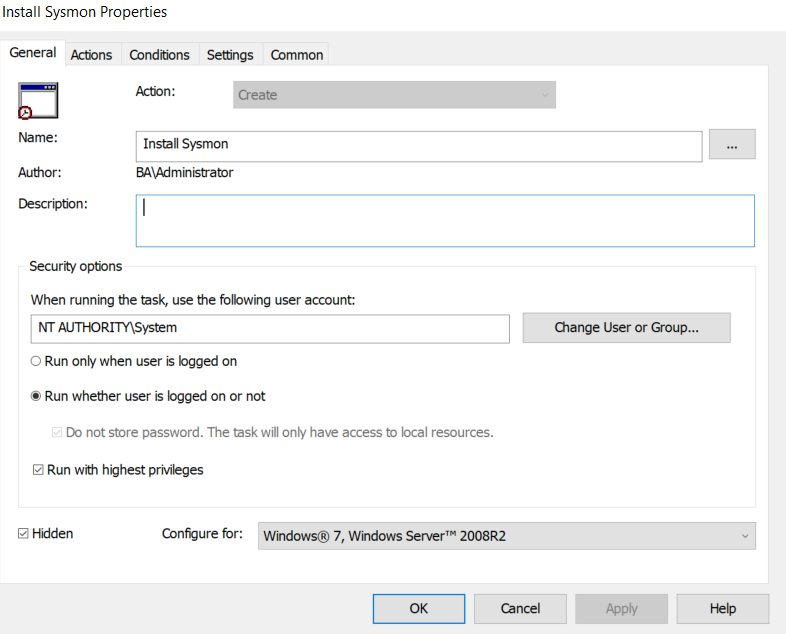
\includegraphics[width=\linewidth]{../img/sysmon/scheduled-task-general.png}
        \caption{Einstellungen Immidiate Task 1}
    \end{figure}

\end{minipage}
\begin{minipage}{0.5\linewidth}
    \begin{figure}[H]
        \centering
        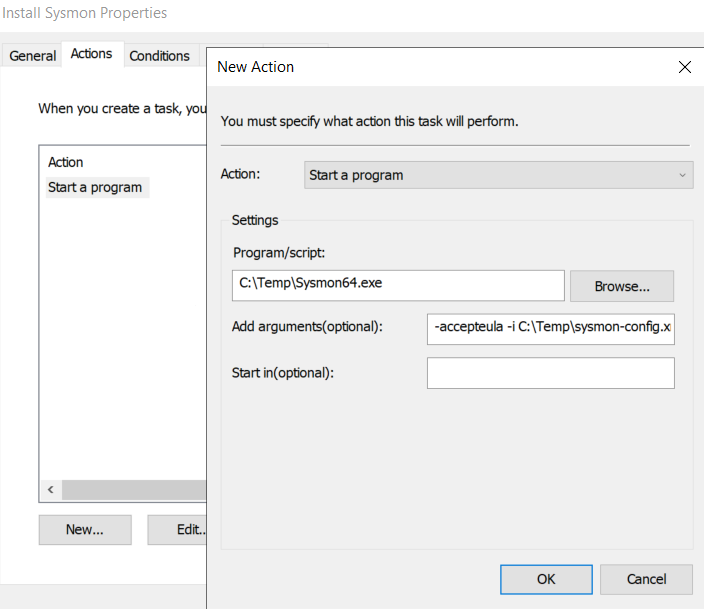
\includegraphics[width=\linewidth]{../img/sysmon/scheduled-task-action.png}
        \caption{Einstellungen Immidiate Task 2}
    \end{figure}
\end{minipage}\\

\textbf{Add Arguments:}
\begin{lstlisting}
-accepteula -i C:\Temp\sysmon-config.xml
\end{lstlisting}

Die Group Policy ist bereit und kann geschlossen werden.
Sysmon wird beim Einloggen auf den Windows Geräten installiert.

\section{Manuelle Installation}
Um Sysmon manuell auf einem Windows Gerät zu installieren, muss man, wie im vorherigen Kapitel beschrieben, die Dateien herunterladen.
Die Konfigurationsdatei kann in das gleiche Verzeichnis wie die .exe kopiert werden.
Danach öffnet man die Kommandozeile als Administrator und wechselt in das Verzeichnis der heruntergeladenen und entpackten Dateien.
Dort gibt man folgendes Kommando ein:
\begin{lstlisting}
    sysmon64.exe -accepteula -i sysmon-config.xml
\end{lstlisting}

Sysmon wird nun auf dem Windows Gerät installiert.